\section{Filtre}
This project utilizes two types of filter a FIR (finite inpulse responds) 
filter and an IIR (infinite impulse responds) filter.
The FIR filter is designed and implemented in matlab using the window method.

\subsection{FIR Filter Design}
First step in designing a FIR filter is to design an ideal IIR filter before
trucating it with by multiplying the IIR filter with a finite length window
function. 

By using our spectral analysis from the earlier sections, we qualitatively
decided to make the cutoff frequence $f_{c} = 10$. The sample frequency $f_{s}$
is given from our dataset, $f_{s} = 47.7774$.

Lastly, the filters made order $M = 250$ thus using $250$ filter coefficients. 

\subsubsection{Resolution}
Next step in designing our filter, we determine the frequency resolution
which provides specifications for the FIR transfer function.

\begin{align}
  \label{eq:freqResolution}
  f_{res} &= \frac{f_{s}}{M}
\end{align}

\subsubsection{Transfer function}
Using $f_{res}$ and $f_{c}$, we can determine which frequency bin
corresponds to frequencies below $f_c$.
This must be in done in integer values i.e.\ rounded to 
closes integer value.

\begin{align}
  \label{eq:freqBin}
  f_{bin} = \left\lfloor\frac{f_{c}}{f_{res}}\right\rfloor = 52
\end{align}

In this case the bin number corresponds to $f_c$ is 52, which
we design our lowpass filter around see \autoref{fig:specificatiion}.

These specification help determine which frequencies should be passed and which should be removed. In this case we remove everything above frequency 10.

\begin{figure}[h]
  \centering
  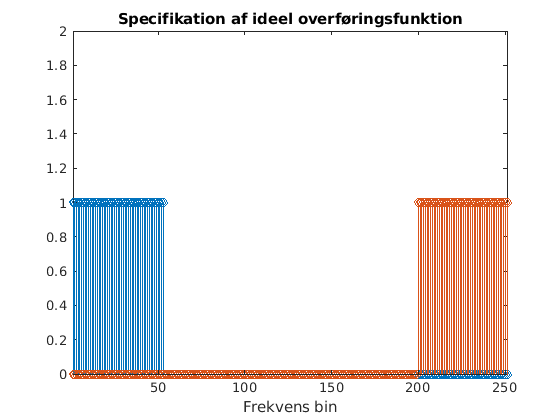
\includegraphics[scale = 0.5]{matlabStuff/Specification_of_transfer_function.png}
  \caption{Specification for our transfor function}%
  \label{fig:specificatiion}
\end{figure}

\newpage

In matlab we can now make our transfer function $h$ using the follwing code. Which when combined with, in our case a hanning window function serves to become our filter which we can run our
data set through.

\begin{figure}[h]
  \centering
  \lstinputlisting[language={matlab}, linerange={27-28,40-40,49-50,58-60}]{matlabStuff/filter.m}
  \caption{matlab code for making a transfer function}%
  \label{}
\end{figure}

Now that we have our transfer function, we can apply it to our data to see if we can reduce the potential noice in data.\
we can plot its coefficients together with the window function, along with the resultat transfer function to see if it
does indeed ``cover'' the peak around $10Hz$.

\begin{figure}[h]
  \centering
  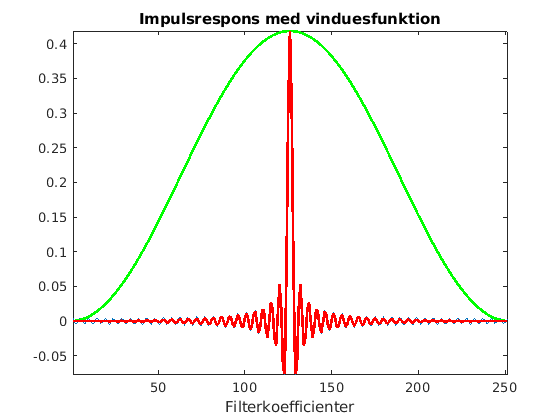
\includegraphics[scale=0.75]{matlabStuff/impulsresponds_with_window.png}
  \caption{Impulseresponds overlayed with the window function, showing its koefficent values as functions of index numbers}%
  \label{fig:impulserespondsWithWindow}
\end{figure}

\newpage

\begin{figure}[h]
  \centering
  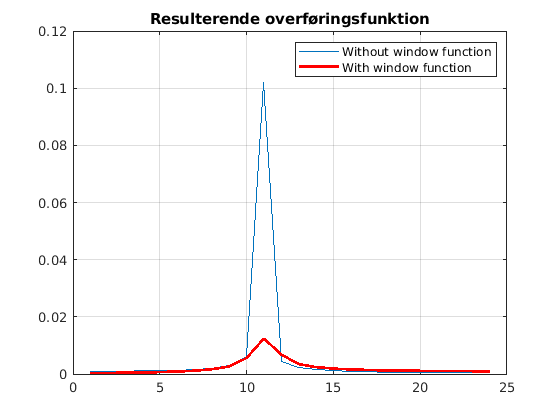
\includegraphics[scale=0.65]{matlabStuff/resuting_transfer_function.png}
  \caption{Resulting transfer function overlayed with and without the window function}%
  \label{fig:resultingTransferFuntion}
\end{figure}

\subsubsection{Applying the FIR filter}
With all of the preperation work done, we can now apply our filter to our dataset to see the results.

\begin{figure}[h]
  \centering
  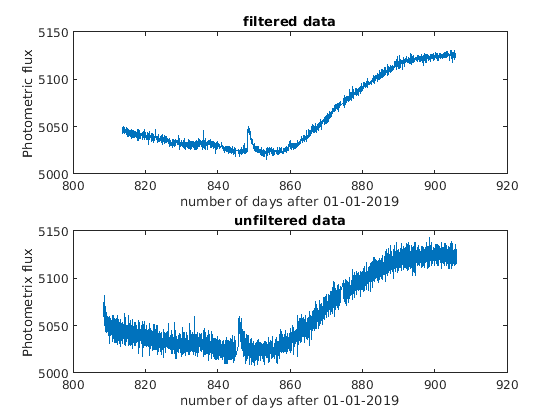
\includegraphics[scale=0.62]{matlabStuff/datasetComparison.png}
  \caption{Side by side comparison of the data before and after the filter has been applied}%
  \label{fig:datasetComparison}
\end{figure}

Its clear fron this comparison that we have manage to remove a some of the signal noice, but since this data set does not show
anything usefull, we wont be able to tell anything from this filtering.


